
\chapter{Aerolites}

\lettrine[lines=4]{\goudy F}rom{} comets I would pass to the consideration of a far more enigmatical class of agglomerated matter - the smallest of all asteroids, to which we apply the name aerolites, or meteoric stones.\footnote{[Much valuable information may be obtained regarding the origin and composition of aerolites or meteoric stones in Memoirs on the subject, by Baumbeer and other writers, in the numbers of Poggendorf Annalen, from 1845 to the present time.] -- Tr.} When they reach our atmosphere in a fragmentary condition, if I should seem to dwell on the specific enumeration of these bodies, and of comets, longer than the general nature of this work might warrant, I have not done so undesignedly. The diversity existing in the individual characteristics of comets has already been noticed. The imperfect knowledge we possess of their physical character renders it difficult, in a work like the present, to give the proper degree of circumstantiality to the phenomena, which, although of frequent recurrence, have been observed with such various degrees of accuracy, or to separate the necessary from the accidental. It is only with respect to measurements and computations that the astronomy of comets has made any marked advancement, and, consequently, a scientific consideration of these bodies must be limited to a specification of the difference in physiognomy and conformation in the nucleus and tail, the instances of great approximation to other cosmical bodies, and of the extremes in the length of their orbits and in their periods of revolution. A faithful delineation of these phenomena, as well as of those which we proceed to consider, can only be given by sketching individual features with the animated circumstantiality of reality. Shooting stars, fireballs, and meteoric stones are, with great probability, regarded as small bodies moving with planetary velocity, and revolving in obedience to the laws of general gravity in conic sections around the Sun. When these masses meet the Earth in their course, and are attracted by it, they enter within the limits of our atmosphere in a luminous condition, and frequently let fall more or less strongly heated stony fragments, covered with a shining black crust. When we enter into a careful investigation of the facts observed at those epochs when showers of shooting stars fell periodically in Cumana in 1799, and in North America during the years 1833 and 1834, we shall find that fireballs can not be considered separately from shooting stars. Both these phenomena are frequently not only simultaneous and blended together, but they likewise are often found to merge into one another, the one phenomenon gradually assuming the character of the other alike with respect to the size of their disks, the emanation of sparks, and the velocities of their motion. Although exploding smoking luminous fireballs are sometimes seen, even in the brightness of tropical daylight,\footnote{A friend of mine, much accustomed to exact trigonometrical measurements, was in the year 1788 at Popayan, a city which is 2 26 north latitude, lying at an elevation of 5583 feet above the level of the sea, and at noon, when the sun was shining brightly in a cloudless sky, saw his room lighted up by a fireball. He had his back to the window at the time, and on turning round, perceived that great part of the path traversed by the fireball was still illuminated by the brightest radiance. Different nations have had the most various terms to express these phenomena - the Germans use the word Sternschnuppe, literally star snuff, an expression well suited to the physical views of the vulgar in foretimes, according to which, the lights in the firmament were said to undergoa process of snuffing or cleaning ; and other nations generally adopt aterm expressive of a shot or fall of stars, as the Swedish stjernjfall, theItalian stella cadente, and the English star shoot. In the woody districtof the Orinoco, on the dreary banks of the Cassiquiare, I heard the natives in the Mission of Vasiva use terms still more inelegant than theGerman star snuff. (Relation Historique du Voy. aux R\'{e}gions Equinoz.,t. ii., p. 513.) These same tribes term the pearly drops of dew whichcover the beautiful leaves of the heliconia star spit. In the Lithuanianmythology, the imagination of the people has embodied its ideas of thenature and signification of falling stars under nobler and more gracefulsymbols. The Parc, Werpeja, weave in heaven for the newbornchild its thread of fate, attaching each separate thread to a star. Whendeath approaches the person, the thread is rent, and the star wanes andsinks to the earth. Jacob Grimm, Deutsche Mythologie, 1843, s. 685.} equaling in size the apparent diameter of the Moon, innumerable quantities of shooting stars have, on the other hand, been observed to fall informs of such extremely small dimensions that they appeatonly as moving points or phosphorescent lines.\footnote{According to the testimony of Professor Denison Olmsted, of YaleCollege, New Haven, Connecticut. (See Poggend., Annalen der Physik,bd. xxx., s. 194.) Kepler, who excluded fireballs and shooting starsfrom the domain of astronomy, because they were, according to hisviews, meteors arising from the exhalations of the earth, and blending with the higher ether, expresses himself, however, generally withmuch caution. He says  Stelle cadentes sunt materia viscida inflammata. Earum alique inter cadendum absumuntur, alique vere in terramcadunt, pondere suo tracte. Nec est dissimile vero, quasdam conglobatasesse ex materia feculentd, in ipsam auram etheream immizta exqueatheris regione, tractu rectilineo, per a\'{e}rem trajicerc, ceu minutos cometas, occult\'{e} causa motus utrorumque.Kepler, Epit. Astron. Copernican, t.i., p. 80.}

It still remains undetermined whether the many luminous bodies that shoot across the sky may not vary in their nature. On my return from the equinoctial zones, I was impressed with an idea that in the torrid regions of the tropics I had more frequently than in our colder latitudes seen shooting stars fall as if from a height of twelve or fifteen thousand feet; that they were of brighter colors, and left a more brilliant line of light in their track; but this impression was no doubt owing to the greater transparency of the tropical atmosphere.\footnote{Relation Historique, t. i., p. 80, 213, 527. If in falling stars, as in comets, we distinguish between the head or nucleus and the tail, we shall find that the greater transparency of the atmosphere in tropical climates is evinced in the greater length and brilliancy of the tail which may be observed in those latitudes. The phenomenon is therefore not necessarily more frequent there, because it is oftener seen and continues longer visible. The influence exercised on shooting stars by the character of the atmosphere is shown occasionally even in our temperate zone, and at very small distances apart. Wartmann relates that on the occasion of a November phenomenon at two places lying very near each other, Geneva and Aux Planchettes, the number of the meteors counted were as 1 to 7. (Wartmann, M\'{e}m. sur les Etoiles filantes, p17.) The tail of a shooting star (or its train), on the subject of which Brandes has made so many exact and delicate observations, is in no way to be ascribed to the continuance of the impression produced by light on the retina. It sometimes continues visible a whole minute, and in some rare instances longer than the light of the nucleus of the shooting star; in which case the luminous track remains motionless. (Gilb., Ann., bd. xiv., 8.251.) This circumstance further indicates the analogy between large shooting stars and fireballs. Admiral Krusenstern saw, in his voyage round the world, the train of a fireball shine for an hour after the luminous body itself had disappeared, and scarcely move throughout the whole time. (Reise, th. i., 8. 58.) Sir Alexander Burnes gives a charming description of the transparency of the clear atmosphere of Bokhara, which was once so favorable to the pursuit of astronomical observations. Bokhara is situated in 39 43 north latitude, and at an elevation of 1280 feet above the level of the sea. There is a constant serenity in its atmosphere, and an admirable clearness in the sky. At night, the stars have uncommon luster, and the Milky Way shines gloriously in the firmament. There is also a never-ceasing display of the most brilliant meteors, which dart like rockets in the sky; ten or twelve of them are sometimes seen in an hour, assuming every color - fiery red, blue, pale, and faint. It is a noble country for astronomical science, and great must have been the advantage enjoyed by the famed observatory of Samarkand. (Burnes, Travels into Bokhara, vol. ii. (1834), p. 158.) A mere traveler must not be reproached for calling ten or twelve shooting stars in an hour many, since it is only recently that we have learned, from careful observations on this subject in Europe, that eight is the mean number which may be seen in an hour in the field of vision of one individual (Quetelet, Corresp. Math\'{e}m., Novem., 1837, p. 447); this number is, however, limited to five or six by that aitigamt observer, Olbers. (Schum., Jahrb., 1838, s. 325.)}
The connection of meteoric stones with the grander phenomenon of fireballs, the former being known to be projected from the latter with such force as to penetrate from ten to fifteen feet into the earth, has been proved, among many other instances, in the falls of a\'{e}rolites at Barbotan, in the Department des Landes (24th July, 1790), at Siena (16th June, 1794), at Weston, in Connecticut, U.S. (14th December, 1807), and at Juvenas, in the Department of Ard\'{e}che (15th June, 1821). Meteoric stones are in some instances thrown from dark clouds suddenly formed in a clear sky, and fall with a noise resembling thunder. Whole districts have thus occasionally been covered with thousands of fragmentary masses, of uniform character but unequal magnitudes, that have been hurled from one of these moving clouds. In less frequent cases, as in that which occurred on the 16th of September, 1843, at Kleinwenden, near Miihlhausen, a large a\'{e}rolite fell with a thundering crash while the sky was clear and cloudless. The intimate affinity between fireballs and shooting stars is further proved by the fact that fireballs, from which meteoric stones have been thrown, have occasionally been found, as at Angers, on the 9th of June, 1822, having a diameter scarcely equal to that of the small fireworks called Roman candles.

The formative power, and the nature of the physical and chemical processes involved in these phenomena, are questions all equally shrouded in mystery, and we are as yet ignorant whether the particles composing the dense mass of meteoric stones are originally, as in comets, separated from one another in the form of vapor, and only condensed within the fiery ball when they become luminous to our sight, or whether, in the case of smaller shooting stars, any compact substance actually falls, or, finally, whether a meteor is composed only of a smoke-like dust, containing iron and nickel; while we are wholly ignorant of what takes place within the dark cloud from which a noise like thunder is often heard for many minutes before the stones fall.\footnote{On meteoric dust, see Arago, in the Annuaire for 1832, p. 254. I have very recently endeavored to show, in another work (Aste Centrale, t.i., p. 408), how the Scythian saga of the sacred gold, which fell burning from heaven, and remained in the possession of the Golden Horde of the Paralatw (Herod., iv., 57), probably originated in the vague recollection of the fall of an a\'{e}rolite. The ancients had also some strange fictions (Dio Cassius, lxxv., 1259) of silver which had fallen from heaven, and with which it had been attempted, under the Emperor Severus, to cover bronze coins; metallic iron was, however, known to exist in meteoric stones. (Plin., ii., 56.) The frequently recurring expression apidibus pluit must not always be understood to refer to falls of a\'{e}rolites. In Liv., xxv.,7, it probably refers to pumice (rapilli) ejected from the volcano, Mount Albanus (Monte Cavo), which was not wholly extinguished at the time. (See Heyne, Opuscula Aeccd., t. iii., p 261; and my Relation. Hist., t.i., p.394.) The contest of Hercules with the Ligyans, on the road from the Caucasus to the Hesperides, belongs to a different sphere of ideas, being an attempt to explain mythically the origin of the round quartz blocks in the Ligyan field of stones at the mouth of the Rhone, which Aristotle supposes to have been ejected from a fissure during an earthquake, and Posidonius to have been caused by the force of the waves of an inland piece of water. In the fragments that we still possess of the play of Aschylus, the Prometheus Delivered, everything proceeds, however, in part of the narration, as in a fall of a\'{e}rolites, for Jupiter draws together a cloud, and causes the district around to be covered by a shower of round stones. Posidonius even ventured to deride the geognostic myth of the blocks and stones. The Lygian field of stones was, however, very naturally and well described by the ancients. The district is now known as La Craw. (See Guerin, Mesures Barom\'{e}triques dans les Alpes, et M\'{e}t\'{e}orologie Avignon, 1829, chap. xii., p. 115.)}

We can ascertain by measurement the enormous, wonderful, and wholly planetary velocity of shooting stars, fireballs, and meteoric stones, and we can gain a knowledge of what is the general and uniform character of the phenomenon, but not of the genetically cosmical process and the results of the metamorphoses. If meteoric stones while revolving in space are already consolidated into dense masses,\footnote{The specific weight of aerolites varies from 19 (Alais) to 43 (Tabor). Their general density may be set down as 3, water being 1. As to what has been said in the text of the actual diameters of fireballs, we must remark, that the numbers have been taken from the few measurements that can be relied upon as correct. These give for the fireball of Weston, Connecticut (14th December, 1807), only 500; for that observed by Le Roi (10th July, 1771) about 1000, and for that estimated by Sir Charles Blagden (18th January, 1783) 2600 feet in diameter. Brandes (Unterhaltungen, bd. i., 8. 42) ascribes a diameter varying from 80 to 120 feet to shooting stars, and a luminous train extending from 12 to 16 miles. There are, however, ample optical causes for supposing that the apparent diameter of fireballs and shooting stars has been very much overrated. The volume of the largest fireball yet observed cannot be compared with that of Ceres, estimating this planet to have a diameter of only 72 English miles. (See the generally so exact and admirable treatise, On the Connection of the Physical Sciences, 1835, p. 411.) With the view of elucidating what has been stated in the text regarding the large aerolite that fell into the bed of the River Narni, but has not again been found, I will give the passage made known by Pertz, from the Chronicon Benedicti, Monacht Sancti Andree in Monte Soracte, a MS. belonging to the tenth century, and preserved in the Chigi Library at Rome. The barbarous Latin of that age has been left unchanged. Anno 921, temporibus domini Johannis Decimi pape, in anno pontificatus illius 7 visa sunt signa. Nam juxta urbem Romam lapides plurimi de calo cadere visi sunt. In civitate que vocatur Narnia tam dirt ac tetri, ut nihil aliud credatur, quam de infernalibus locis deducti essent. Nam ita ex illis lapidibus unus omnium maximus est, ut drcidensin flumen Narnus, ad mensuram unius cubiti super aquas fluminis usque hodie videretur. Nam et ignite facule de celo plurime omnibus in hac civitate Romani populi vise sunt, ita ut pene terra contingeret. Alia cadentes, c. (Pertz, Monum. Germ. Hist. Scriptores, t. iii., p. 715.) On the aerolites of gos Potamos, which fell, according to the Parian Chronicle, in the 78 1 Olympiad, see Béckh, Corp. Inscr. Graec., t. ii., p. 302, 320, 340; also Aristot., Meteor., i., 7 (Idelers Comm., t. 1., p. 404-407); Stob., Hcl. Phys., 1, 25, p. 508 (Heeren); Plut., Lys., c. 12; Diog. Laert., ii., 10; and see, also, subsequent notes in this work. According to a Mongolian tradition, a black fragment of a rock, forty feet in height, fell from heaven on a plain near the source of the Great Yellow River in Western China. (Abel Rémusat, in Lamétherie, Jour. de Phys., 1819, Mai, p. 264.)} less dense, however, than the mean density of the earth, they must be very small nuclei, which, surrounded by inflammable vapor or gas, form the innermost part of fireballs, from the height and apparent diameter of which we may, in the case of the largest, estimate that the actual diameter varies from 500 to about 2800 feet. The largest meteoric masses as yet known are those of Otumpa, in Chaco, and of Bahia, in Brazil, described by Rubi de Celis as being from 7 to 74 feet in length. The meteoric stone of Aagos Potamos, celebrated in antiquity, and even mentioned in the Chronicle of the Parian Marbles, which fell about the year in which Socrates was born, has been described as of the size of two millstones, and equal in weight to a full wagon load. Notwithstanding the failure that has attended the efforts of the African traveler, Brown, I do not wholly relinquish the hope that, even after the lapse of 2312 years, this Thracian meteoric mass, which it would be so difficult to destroy, may be found, since the region in which it fell is now become so easy of access to European travelers. The huge aerolite which in the beginning of the tenth century fell into the river at Narni, projected between three and four feet above the surface of the water, as we learn from a document lately discovered by Pertz. It must be remarked that these meteoric bodies, whether in ancient or modern times, can only be regarded as the principal fragments of masses that have been broken up by the explosion either of a fireball or a dark cloud.

\begin{figure}[htbp]
  \centering
  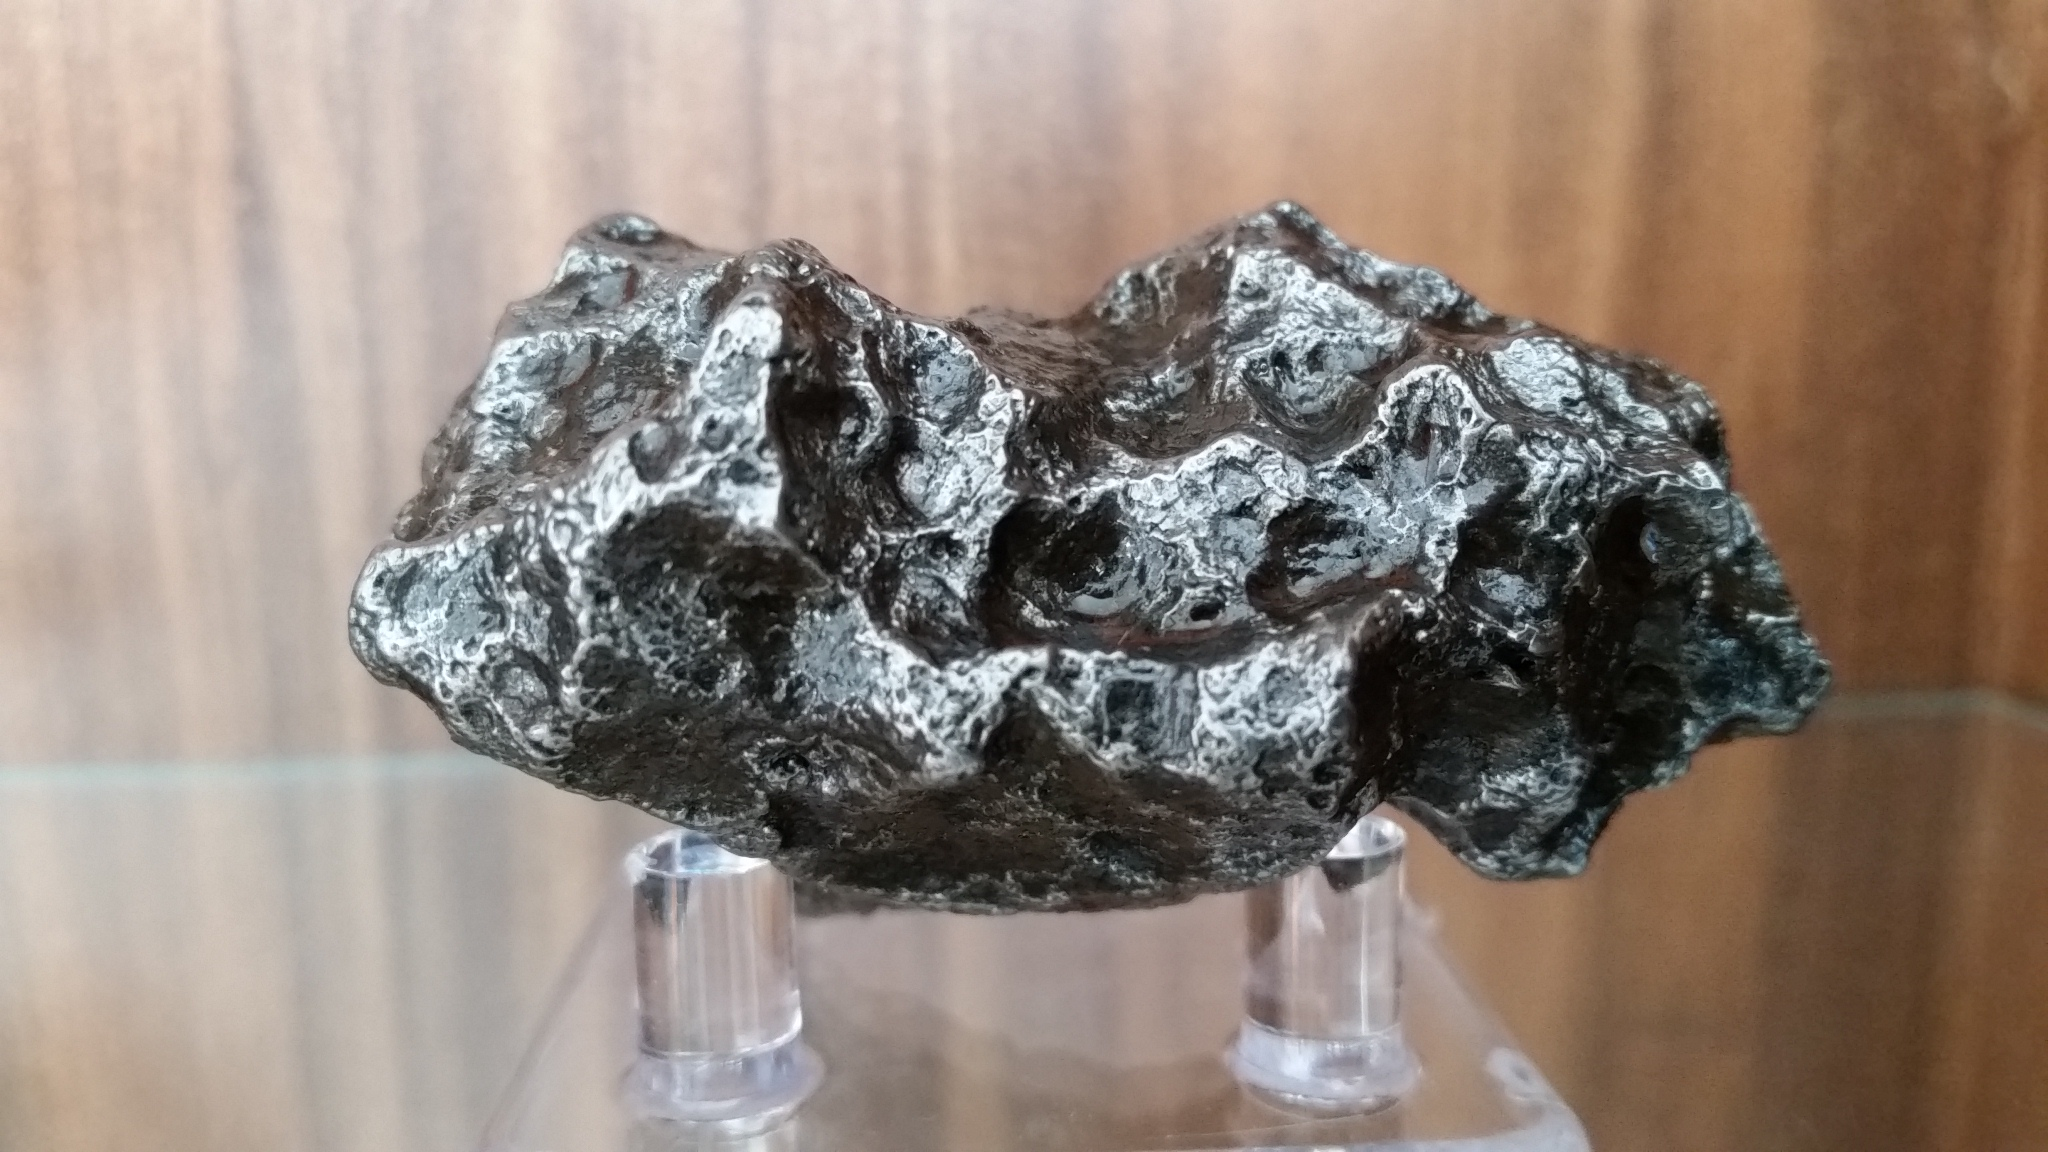
\includegraphics[width=1\textwidth]{../../pictures/Campo_del_Cielo_Museum_Grade_275_grams.jpg}
  \caption{Fragment of El Chaco meteorite. Licensed under \href{https://creativecommons.org/licenses/by-sa/4.0/deed.en}{CC-BY-SA 4.0}. Author: \href{https://commons.wikimedia.org/wiki/File:Campo_del_Cielo_Museum_Grade_275_grams.jpg}{Howardites Meteorites}}
  \label{fig:figure_label}
\end{figure}

On considering the enormous velocity with which, as hasbeen mathematically proved, meteoric stones reach the earthfrom the extremest confines of the atmosphere, and the lengthened course traversed by fireballs through the denser strataof the air, if seems more than improbable that these metalliferous stony masses, containing perfectlyformed erystals of olivine, labradorite, and pyroxene, should in so short a period oftime have been converted from a vaporous condition to a solidnucleus. Moreover, that which falls from meteoric masses,even where the internal composition is chemically different,exhibits almost always the peculiar character of a fragment,being of a prismatic or truncated pyramidal form, with broad,somewhat curved faces, and rounded angles. But whencecomes this form, which was first recognized by Schreiber ascharacteristic of the severed part of a rotating planetary body Here, as in the sphere of organic life, all that appertains tothe history of development remains hidden in obscurity. Meteoric masses become luminous and kindle at heights which must be regarded as almost devoid of air, or occupied by atatmosphere that does not even contain y5';;5th part of oxygen. The recent investigations of Biot on the important phenomenon of twilight\footnote{Biot, Trait\'{e} d Astronomie Physique (3\'{e}me \'{e}d.), 1841, t.i., p. 149177, 238, 312. My lamented friend Poisson endeavored, in a singularmanner, to solve the difficulty attending an assumption of the spontaneous ignition of meteoric stones at an elevation where the density ofthe atmosphere is almost null. These are his words It is difficult toattribute, as is usually done, the incandescence of atrolites to frictionagainst the molecules of the atmosphere at an elevation above the earthwhere the density of the air is almost null. May ve not suppose thatthe electric fluid, in a neutral condition, forms a kind of atmosphere, extending far beyond the mass of our atmosphere, yet subject to terrestrial attraction, although physically imponderable, and consequently following our globe in its motion According to this hypothesis, thebodies of which we have been speaking would, on entering this imponderable atmosphere, decompose the neutral fluid by their unequalaction on the two electricities, and they would thus be heated, and ina state of incandescence, by becoming electrified. (Poisson, Rech. surla Probabilit\'{e} des Jugements, 1837, p. 6.)} have considerably lowered the lineswhich had, perhaps with some degree of temerity, been usually termed the boundaries of the atmosphere; but processes oflight may be evolved independently of the presence of oxygen,and Poisson conjectured that a\'{e}rolites were ignited far beyondthe range of our atmosphere. Numerical calculation and geometrical measurement are the only means by which, as in thecase of the larger bodies of our solar system, we are enabled toimpart a firm and safe basis to our investigations of meteoricstones. Although Halley pronounced the great fireball of 1686,whose motion was opposite to that of the earth in its orbit,\footnote{Philos. Transact., vol. xxix., p. 161163. .} tobe a cosmical body, Chladni, in 1794, first recognized, withready acuteness of mind, the connection between fireballs andthe stones projected from the atmosphere, and the motions of theformer bodies in space.\footnote{The first edition of Chladnis important treatise, Ueber den Ursprung der von Pallas gefundenen und anderen Eisenmassen (On theOrigin of the masses of Iron found by Pallas, and other similar masses),appeared two months prior to the shower of stones at Siena, and twyears before Lichtenberg stated, in the Gottingen Taschenbuch, thastones reach our atmosphere from the remoter regions of space.Comp., also, Olberss letter to Benzenberg, 18th Nov., 1837, in Benzenbergs T'reatise on Shooting Stars, p. 186} A brilliant confirmation of the cosmical origin of these phenomena has been afforded by DenisonOlmsted, at New Haven, Connecticut, who has shown, on theconcurrent authority of all eyewitnesses, that during the celebrated fall of shooting stars on the night between the 12th and 13th of November, 1833, the fireballs and shooting starsall emerged from one and the same quarter of the heavens,namely, in the vicinity of the star y in the constellation Leo,and did not deviate from this point, although the star changedits apparent height and azimuth during the time of the observation. Such an independence of the Earths rotation showsthat the luminous body must have reached our atmosphere fromwithout. According to Enckes computation\footnote{Encke, in Poggend., Annalen, bd. xxxiii. (1834), s. 213. Arago,in the Annuaire for 1836, p. 291. Two letters which I wrote to Benzenberg, May 19 and October 22, 1837, on the conjectural precessionof the nodes in the orbit of periodical falls of shooting stars. (Benzenbergs Sternsch., s. 207 and 209.) Olbers subsequently adopted thisopinionof the gradual retardation of the November phenomenon(Astron. Nachr., 1838, No. 372, 8. 180.) If I may venture to combinetwo of the falls of shooting stars mentioned by the Arabian writerswith the epochs found by Boguslawski for the fourteenth century, Iobtain the following more or less accordant elements of the movementsof the nodes: 
 
 In Oct., 902, on the night in which King Ibrahim ben Ahmed died,there fell a heavy shower of shooting stars, like a fiery rain; andthis year was, therefore, called the year of stars. (Conde, Hist. de laDomin. de los Arabes, p. 346.)
 
 On the 19th of Oct., 1202, the stars were in motion all night.  Theytell like locusts. (Comptes Rendus, 1837, t. i., p.294; and Freehn, inthe Bull. de 7 Acad\'{e}mie de St. P\'{e}tersbourg, t. iii., p. 308.)
 
 On the 2st Oct., O.S., 1366,  die sequente post festum XI. millia Virginum ab hora matutina usque ad horam primam vise sunt quasi stellade calo cadere continuo, et in tanta multitudine, quod nemo narrare sufjicit. This remarkable notice, of which we shall speak more fully inthe subsequent part of this work, was found by the younger Von Boguslawski, in Benesse (de ee de Weitmil or Weithmiil, Chrontcon Ecclesiae Pragensis, p. 389. This chronicle may also be found inthe second part of Scriptores rerum Bohemicarum, by Pelzel and Dobrowsky, 1784. (Schum., Astr. Nachr., Dec., 1839.)
 
 On the night between the 9th and 10th of November, 1787, many falling stars were observed at Manheim, Southern Germany, by Hemmer(Kamtz, Meteor., th. iii., s. 237.)
 
 After midnight, on the 12th of November, 1799, occurred the extraordinary fall of stars at Cumana, which Bonpland and myself have described, and which was observed over a great part of the earth. (RelatHist., t. i., p. 519527.)
 
 Between the 12th and 13th of November, 1822, shooting stars, inter.mingled with fireballs, were seen in large numbers by Kloden, atPotsdam. (Gilberts Anz., bd. xxii., s. 291.)
 
 On the 13th of November, 1831, at 4 oclock in the morning, a greatshower of falling stars was seen by Captain B\'{e}rard, on the Spanishcoast, near Carthagena del Levante. (Annuaire, 1836, p. 297.)
 
 In the night between the 12th and 13th of November, 1833, occurredthe phenomenon so admirably described by Professor Olmsted, inNorth America.
 
 Tn the night of the 1314th of November, 1834, a similar fall of shooting stars was seen in North America, although the numbers were notquite so considerable. (Poggend., Annalen, bd. xxxiv., s. 129.)
 
 On the 13th of November, 1835, a barn was set on fire by the fall ofa sporadic fireball, at Belley, in the Department de lAin. (Annuaire,1836, p. 296.)
 
 In the year 1838, the stream showed itself most decidedly on thenight of the 1314th of November. (Astron. Nachr., 1838, No. 372.)
 } of the whole number of observations made in the United States of NorthAmerica, between the thirtyfifth and the fortysecond degreesof latitude, it would appear that all these meteors came fromthe same point of space in the direction in which the Earthwas moving at the time. On the recurrence of falls of shooting stars in North America, in the month of November of theyears 1834. and 1837, and in the analogous falls observed atBremen in 1838, a like general parallelism of the orbits, andthe same direction of the meteors from the constellation Leo,were again noticed. It has been supposed that a greaterparallelism was observable in the direction of periodic falls ofshooting stars than in those of sporadic occurrence ; and it hasfurther been remarked, that in the periodicallyrecurring fallsin the month of August, as, for instance, in the year 1839, whemeteors came principally from one point between Perseus andTaurus, toward the latter of which constellations the Earthwas then moving. This peculiarity of the phenomenon, manifested in the retrograde direction of the orbits in Novemberand August, should be thoroughly investigated by accurateobservations, in order that it may either be fully confirmed or refuted.

The heights of shooting stars, that is to say, the heights of the points at which they begin and cease to be visible, vary exceedingly, fluctuating between 16 and 140 miles. This important result, and the enormous velocity of these problematical asteroids, were first ascertained by Benzenberg and Brandes, by simultaneous observations and determinations of parallax at the extremities of a base line of 49,020 feet in length.\footnote{I am well aware that, among the 62 shooting stars simultaneously observed in Silesia, in 1823, at the suggestion of Professor Brandes some appeared to have an elevation of 183 to 240, or even 400 miles. (Brandes, Unterhaltungen für Freunde der Astronomie und Physik, hefti., s. 48. Instructive Narratives for the Lovers of Astronomy and Physics.) But Olbers considered that all determinations for elevations beyond 120 miles must be doubtful, owing to the smallness of the parallax.} The relative velocity of motion is from 18 to 36 miles in a second, and consequently equal to planetary velocity. This planetary velocity,\footnote{The planetary velocity of translation, the movement in the orbit, is in Mercury 264, in Venus 193, and in the Earth 164 miles in a second.} as well as the direction of the orbits of fireballs and shooting stars, which has frequently been observed to be opposite to that of the Earth, may be considered as conclusive arguments against the hypothesis that a\'{e}rolites derive their origin from the so-called active lunar volcanoes. Numerical views regarding a greater or lesser volcanic force on a small cosmical body, not surrounded by any atmosphere, must, from their nature, be wholly arbitrary. We may imagine the reaction of the interior of a planet on its crust ten or even a hundred times greater than that of our present terrestrial volcanoes; the direction of masses projected from a satellite revolving from west to east might appear retrogressive, owing to the Earth in its orbit subsequently reaching that point of space at which these bodies fall. If we examine the whole sphere of relations which I have touched upon in this work, in order to escape the charge of having made unproved assertions, we shall find that the hypothesis of the selenic origin of meteoric stones\footnote{Chladni states that an Italian physicist, Paolo Maria Terzago, onthe occasion of the fall of an a\'{e}rolite at Milan in 1660, by which a Franciscan monk was killed, was the first who surmised that a\'{e}rolites wereof selenic origin. He says, in a memoir entitled Museum Septalianum,Manfredi Septale, Patricit Mediolanensis, industrioso labore constructumTortona, 1664, p. 44), Labant philosophorum mentes sub horum lapidumponderibus; ni dicire velimus, lunam terram alteram, sine mundum esse,ex cujus montibus divisa frustra in inferiorem nostrum hunc orbem delabantur. Without any previous knowledge of this conjecture, Olberswas led, in the year 1795 (after the celebrated fall at Siena on the 16thof June, 1794), into an investigation of the amount of the initial tangential force that would be requisite to bring to the Earth masses projected from the Moon. This ballistic problem occupied, during ten ortwelve years, the attention of the geometricians Laplace, Biot, Brandes,and Poisson. The opinion which was then so prevalent, but which hassince been abandoned, of the existence of active volcanoes in the Moon,where air and water are absent, led to a confusion in the minds of thegenerality of persons between mathematical possibilities and physicalprobabilities. Olbers, Brandes, and Chladni thought  that the velocityof 16 to 32 miles, with which fireballs and shooting stars entered ouratmosphere, furnished a refutation to the view of their selenic origin.According to Olbers, it would require to reach the Earth, setting asidethe resistance of the air, an initial velocity of 8292 feet in the second 5according to Laplace, 7862 ; to Biot, 8282; and to Poisson, 7595. Laplace states that this velocity is only five or six times as great as that ofacannon ball; but Olbers has shown  that, with such an initial veloc.ity as 7500 or 8000 feet in a second, meteoric stones would arrive at thesurface of our earth with a velocity of only 35,000 feet (or 153 Germangeographical mile). But the measured velocity of meteoric stones averages five such miles, or upward of 114,000 feet to a second; and,consequently, the original velocity of projection from the Moon mustbe almost 110,000 feet, and therefore fourteeu times greater than Laplace asserted. (Olbers, in Schum., Jahrd., 1837, p. 5258; and in Gehler, Neues Physik. Worterbuche, bd. vi., abth. 3, s. 21292136.) Ifwe could assume volcanic forces to be still active on the Moons surface,the absence of atmospheric resistance would certainly give to theirprojectile force an advantage over that of our terrestrial volcanoes; buteven in respect to the measure of the latter force (the projectile forceof our own volcanoes), we have no observations on which any reliancecan be placed, and it has probably been exceedingly overrated. Dr.Peters, who accurately observed and measured the phenomena .presented by tna, found that the greatest velocity of any of the stones projected from the crater was only 1250 feet toa second. Observationson the Peak of Teneriffe, in 1798, gave 3000 feet. Although Laplace,at the end of his work (Expos. du Syst. du Monde, ed. de 1824, p. 399),cautiously observes, regarding a\'{e}rolites, that in all probability theycome from the depths of space, yet we see from another passage(chap. vi., p. 233) that, being probably unacquainted with the extraordinary planetary yelocity of meteoric stones, he inclines to the hypothesis of their lunar origin, always, however, assuming that the stonesprojected from the Moon become satellites of our Earth, describingaround it more or less eccentric orbits, and thus not reaching its atmosphere until several or even many revolutions have been accomplished.As an Italian at Tortona had the fancy that a\'{e}rolites came from theMoon, so some of the Greek philosophers thought they came from theSun. This was the opinion of Diogenes Laertius (ii., 9) regarding theorigin of the mass that fell at A.gos Potamos (see note, p. 116). Pliny,whose labors in recording the opinions and statements of precedingwriters are astonishing, repeats the theory, and derides it the morefreely, because he, with earlier writers (Diog. Laert., 3 and 5, p. 99,Hibner), accuses Anaxagoras of having predicted tlie fall of a\'{e}rolitesfrom the Sun Celebrant Greci Anaxagoram Clazomenium Olympiadis septuagesime octave secundo anno predixisse celestiam litterarum scientia, quibus diebus saxum casurum esse e sole, idque factuminterdiu in Thracie parte ad Agos flumen. Quod si quis predictumcredat, simul fateatur necesse est, majoris miraculi divinitatem Anaxagore fuisse, solvique rerum nature intellectum, et confundi omnia, siaut ipse Sol lapis esse aut unquam lapidem in eo fuisse credatur; decidere tamen crebro non erit dubium. The fall of a moderatesizedstone, which is preserved in the Gymnasium at Abydos, is also reperted to have been foretold by Anaxagoras. The fall of a\'{e}rotites in brightsunshine, and when the Moons disk was invisible, probably led to theidea of sunstones. Moreover, according to one of the physical dogmasof Anaxagoras, which brought on him the persecution of the theologians(even as they have attacked the geologists of our own times), the Sunwas regarded as (a molten fiery mass (u\'{e}dpoc dtdtupoc). In accordance with these views of Anaxagoras, we find Euripides, in Phagton,terming the Sun a golden mass; that is to say, a firecolored, brightlyshining matter, but not leading to the inference that a\'{e}rolites aregolden sunstones. (See note to page 115.) Compare Valckenaer,Diatribe in Eurip. perd. Dram. Reliquias, 1767, p. 30. Diog. Laert.,ii, 40. Hence, among the Greek philosophers, we find four hypothesesregarding the origin of falling stars a telluric origin from ascendingexhalations; masses of stone raised by hurricane (see Aristot., Meteor.,lib. i., cap. iv., 213, and cap. vii., 9); a solar origin; and, lastly, an origin in the regions of space, as heavenly bodies which had long remained invisible. Respecting this last opinion, which is that of Diogenes of Apollonia, and entirely accords with that of the present day,see pages 124 and 125. Itis worthy of remark, that in Syria, as I havebeen assured by a learned Orientalist, now resident at Smyrna, Andreade Nericat, who instructed me in Persian, there is a popular belief thata\'{e}rolites chiefly fall on clear moonlight nights. The ancients, on thecontrary, especially looked for their fall during lunar eclipses. (SeePliny, xxxvil., 10, p. 164. Solinus, c. 37. Salm., Ezere., p. 531; andthe passages collected by Ukert, in his Geogr. der Griechen und R\'{e}mer,th. ii., 1, 8. 331, note 14.) On the improbability that meteoric massesare formed from metaldissolving gases, which, according to Fusinieri,may exist in the highest strata of our atmosphere, and, previously diffused through an almost boundless space, may suddenly assume a solidcondition, and on the penetration and misceability of gases, see myRelat. Hist., t. i., p. 525.
} depends upon a number of conditions. whose accidental coincidence could alone convert a possibleinto an actual fact. The view of the original existence of small planetary masses in space is simpler, and, at the sametime, more analogous with those entertained concerning theformation of other portions of the solar system.

It is very probable that a large number of these cosmic bodies traverse space undestroyed by the vicinity of our atmosphere, and revolve around the Sun without experiencing any alteration but a slight increase in the eccentricity of their orbits, occasioned by the attraction of the Earth's mass. We may, consequently, suppose the possibility of these bodies remaining invisible to us during many years and frequent revolutions. The supposed phenomenon of ascending shooting stars and fireballs, which Chladni has unsuccessfully endeavored to explain on the hypothesis of the reflection of strongly compressed air, appears at first sight as the consequence of some unknown tangential force propelling bodies from the earth; but Bessel has shown by theoretical deductions, confirmed by Feldt's carefully conducted calculations, that, owing to the absence of any proofs of the simultaneous occurrence of the observed disappearances, the assumption of an ascent of shooting stars was rendered wholly improbable, and inadmissible as a result of observation.\footnote{Bessel, in Schum., Asir. Nachr., 1839, No 380 und 381, s. 222 und 346. At the conclusion of the Memoir there is a comparison of the Sun's longitudes with the epochs of the November phenomenon, from the period of the first observations in Cumana in 1798} The opinion advanced by Olbers that the explosion of shooting stars and ignited fireballs not moving in straight lines may impel meteors upward in the manner of rockets, and influence the direction of their orbits, must be made the subject of future researches.

Shooting stars fall either separately and in inconsiderablenumbers, that is, sporadically, or in swarms of many thousands. Ihe latter, which are compared by Arabian authorsto swarms of locusts, are periodic in their occurrence, andmove in streams, generally in a parallel direction. Amongperiodic falls, the most celebrated are that known as the November phenomenon, occurring from about the 12th to the14th of November, and that of the festival of St. Lawrence(the 10th of August), whose fiery tears were noticed informer times in a church calendar of England, no less thanin old traditionary legends, as'a meteorological event of constant recurrence.\footnote{Dr. Thomas Forster (Lhe Pocket Encyclopedia of Natural Phenomena, 1827, p. 17) states that a manuscript is preserved in the library of Christ's College, Cambridge, written in the tenth century by amonk, and entitled Ephemerides Rerum Naturalium, in which the natural phenomena for each day of the year are inscribed, as, for instance,the first flowering of plants, the arrival of birds, c.; the 10th of August is distinguished by the word  meteorodes. It was this indication, and the tradition of the fiery tears of St. Lawrence, that chieflyinduced Dr. Forster to undertake his extremely zealous investigationof the August phenomena. (Quetelet, Correspond. Math\'{e}m., S\'{e}rie II1.,t. 1.,1837, p. 433.) ;} Notwithstanding the great quantity ofshooting stars and fireballs of the most various dimensions,which, according to Kloden, were seen to fall at Potsdam on the night between the 12th and 13th of November, 1822,and on the same night of the year in 1832 throughout thewhole of Europe, from Portsmouth to Orenburg on the UralRiver, and even in the southern hemisphere, as in the Isle ofFrance, no attention was directed to the periodicity of thephenomenon, and no idea seems to have been entertained ofthe connection existing between the fall of shooting stars andthe recurrence of certain days, until the prodigious swarm ofshooting stars which occurred in North America between the12th and 13th of November, 1833, and was observed byOlmsted and Palmer. The stars fell, on this occasion, likeflakes of snow, and it was calculated that at least 240,000had fallen during a period of nine hours. Palmer, of NewHaven, Connecticut, was led, in consequence of this splendidphenomenon, to the recollection of the fall of meteoric stonesin 1799, first described by Ellicot and myself,\footnote{Humb., Rel. Hist., t. i., p. 519527. Ellicot, in the Transactionsof the American Society, 1804, vol. vi., p.29. Arago makes the following observations in reference to the November phenomena  We thusbecome more and more confirmed in the belief that there exists a zonecomposed of millions of small bodies, whose orbits cut the plane of the ecliptic at about the point which our Earth annually occupies betweenthe 11th and 13th of November. It is a new planetary world beginning to be revealed to us. (Annuaire, 1836, p. 296.)

[No such manuscript is at present known to exist in the library of that college.For this information I am indebted to the inquiries of Mr. Cory, of Pembroke Colen a learned editor of Hieroglyphics of Horapollo Nilovs, Greek and English,1840.] -- Tr.

} and which, by a comparison of the facts I had adduced, showed that thaphenomenon had been simultaneously seen in the New Continent, from the equator to New Herrnhut in Greenland (6414 north latitude), and between 46. and 82 longitude.The identity of the epochs was recognized with astonishment.The stream, which had been seen from Jamaica to Boston(40 21 north latitude) to traverse the whole vault of heavenon the 12th and 13th of November, 1833, was again observedin the United States in 1834, on the night between the 13thand 14th of November, although on this latter occasion itshowed itself with somewhat less intensity. In Europe theperiodicity of the phenomenon has since been manifested withgreat regularity.

Another and a like regularly recurring phenomenon is that noticed in the month of August, the meteoric stream of St. Lawrence, appearing between the 9th and 14th of August. Muschenbroek,\footnote{On the 25th of April, 1095, innumerable eyes in France saw stars falling from heaven as thickly as hail (wt grando, nisi lucerent, pro densitate putaretur; Baldr., p. 88), and this occurrence was regarded by the Council of Clermont as indicative of the great movement in Christendom. (Wilken, Gesch. der Kreuzzige, bd. i.,8. 75.) On the 25th of April, 1800, a great fall of stars was observed in Virginia and Massachusetts; it was (a fire of rockets that lasted two hours. Arago was the first to call attention to this train\'{e}e dasteroides, as a recurring phenomenon. (Annuaire, 1836, p. 297.) The falls of a\'{e}rolites in the beginning of the month of December are also deserving of notice. In reference to their periodic recurrence as a meteoric stream, we may mention the early observation of Brandes on the night of the 6th and 7th of December, 1798 (when he counted 2000 falling stars), and very probably the enormous fall of a\'{e}rolites that occurred at the Riv Assu, near the village of Macao, in the Brazils, on the 11th of December, 1836. (Brandes, Unterhalt. fur Freunde der Physik, 1825, heft i., s. 65, and Comptes Rendus, t. v.,p.211.) Capocci, in the interval between 1809 and 1839, a space of thirty years, has discovered twelve authenticated cases of a\'{e}rolites occurring between the 27th and 29th of November, besides others on the 13th of November, the 10th of August, and the 17th of July. (Comptes Rendus, t. xi., p. 357.) It is singular that in the portion of the Earth's path corresponding with the months of January and February, and probably also with March, no periodic streams of falling stars or a\'{e}rolites have as yet been noticed; although, when in the South Sea in the year 1803, I observed on the 15th of March a remarkably large number of falling stars, and they were seen to fall as in a swarm in the city of Quito, shortly before the terrible earthquake of Riobamba on the 4th of February, 1797. From the phenomena hitherto observed, the following epochs seem especially worthy of remark: 22nd to the 25th of April, 17th of July (17th to the 26th of July). (Quet., Corr., 1837, p. 435.) 10th of August, 12th to the 14th of November, 27th to the 29th of November, 6th to the 12th of December. When we consider that the regions of space must be occupied by myriads of comets, we are led by analogy, notwithstanding the differences existing between isolated comets and rings filled with asteroids, to regard the frequency of these meteoric streams with less astonishment than the first consideration of the phenomenon would be likely to excite. ;
} as early as in the middle of the last century, drew attention to the frequency of meteors in the month of August; but their certain periodic return about the time of St. Lawrence's day was first shown by Quetelet, Olbers, and Benzenberg. We shall, no doubt, in time, discover other periodically appearing streams,\footnote{Compare Muschenbroek, Introd. ad Phil. Nat., 1762, t. ii., p. 1061; Howard, On the Climate of London, vol. ii., p. 23, observations of the year 1806; seven years, therefore, after the earliest observations of Brandes (Benzenberg, aber Slernschnuppen, s. 240244); the August observations of Thomas Forster, in Quetelet, op. cit., p. 438453; those of Adolph Erman, Boguslawski, and Kreil, in Schum., Jakrb., 1838, s. 317330. Regarding the point of origin in Perseus, on the 10th of August, 1839, see the accurate measurements of Bessel and Erman (Schum., Astr. Nachr., No. 385 und 428); but on the 10th of August, 1837, the path does not appear to have been retrograde; see Arago, in Comptes Rendus, 1837, t. ti., p. 183.} probably about the 22nd to the 25th of April, between the 6th and 12th of December, and, to judge by the number of true falls of a\'{e}rolites enumerated by Capoccei, also between the 27th and 29th of November, or about the 17th of July.

Although the phenomena hitherto observed appear to have been independent of the distance from the pole, the temperature of the air, and other climatic relations, there is, however, one perhaps accidentally coincident phenomenon which must not be wholly disregarded. The Northern Light, the Aurora Borealis, was unusually brilliant on the occurrence of the splendid fall of meteors of the 12th and 13th November, 1833, described by Olmsted. It was also observed at Bremen in 1838, where the periodic meteoric fall was, however, less remarkable than at Richmond, near London. I have mentioned in another work the singular fact observed by Admiral Wrangel, and frequently confirmed to me by himself,\footnote{Ferd. v. Wrangle, Reise längs der Nordkiste von Sibirien in den Jahren, 1820-1824, th. ii., s. 259. Regarding the recurrence of the denser swarm of the November stream after an interval of thirty-three years, see Olbers, in Jzhrb., 1837, s. 280. I was informed in Cumanathat shortly before the fearful earthquake of 1766; and consequently thirty-three years (the same interval) before the great fall of stars on the 11th and 12th of November, 1799, a similar fiery manifestation had been observed in the heavens. But it was on the 21st of October, 1766, and not in the beginning of November, that the earthquake occurred. Possibly some traveler in Quito may yet be able to ascertain the day on which the volcano of Cayambe, which is situated there, was for the space of an hour enveloped in falling stars, so that the inhabitants endeavored to appease heaven by religious processions. (Relat. Hist., i., chap. iv., p. 307; chap. x., p. 520 and 527.)} that when he was on the Siberian coast of the Polar Sea, he observed, during an Aurora Borealis, certain portions of the vault of heaven, which were not illuminated, light up and continue luminous whenever a shooting star passed over them.

The different meteoric streams, each of which is composed of myriads of small cosmical bodies, probably intersect our Earth's orbit in the same manner as Biela's comet. According to this hypothesis, we may represent to ourselves these asteroid meteors as composing a closed ring or zone, within which they all pursue one common orbit. The smaller planets between Mars and Jupiter present us, if we except Pallas, with an analogous relation in their constantly intersecting orbits. As yet, however, we have no certain knowledge as to whether changes in the periods at which the stream becomes visible, or the retardations of the phenomena of which I have already spoken, indicate a regular precession or oscillation of the nodes—that is to say, of the points of intersection of the Earth's orbit and of that of the ring; or whether this ring or zone attains so considerable a degree of breadth from the irregular grouping and distances apart of the small bodies, that it requires several days for the Earth to traverse it. The system of Saturn's satellites shows us likewise a group of immense width, composed of most intimately connected cosmical bodies. In this system, the orbit of the outermost (the seventh) satellite has such a vast diameter, that the Earth, in her revolution round the Sun, requires three days to traverse an extent of space equal to this diameter. If, therefore, in one of these rings, which we regard as the orbit of a periodical stream, the asteroids should be so irregularly distributed as to consist of but few groups sufficiently dense to give rise to these phenomena; we may easily understand why we so seldom witness such glorious spectacles as those exhibited in the November months of 1799 and 1833. The acute mind of Olbers led him almost to predict that the next appearance of the phenomenon of shooting stars and fireballs intermixed, falling like flakes of snow, would not recur until between the 12th and 14th of November, 1867.

The stream of the November asteroids has occasionally only been visible in a small section of the Earth. Thus, for instance, a very splendid meteoric shower was seen in England in the year 1837, while a most attentive and skillful observer at Braunsberg, in Prussia, only saw, on the same night, which was there uninterruptedly clear, a few sporadic shooting stars fall between seven o'clock in the evening and sunrise the next morning. Bessel\footnote{From a letter to myself, dated Jan. 24th, 1838. The enormous swarm of falling stars in November, 1799, was almost exclusively seen in America, where it was witnessed from New Herrnhut in Greenland to the equator. The swarms of 1831 and 1832 were visible only in Europe, and those of 1833 and 1834 only in the United States of North America.} concluded from this that a dense group of the bodies composing the great ring may have reached that part of the Earth in which England is situated, while the more eastern districts of the Earth might be passing at the time through a part of the meteoric ring proportionally less densely studded with bodies. If the hypothesis of a regular precession or oscillation of the nodes should acquire greater weight, special interest will be attached to the investigation of older observations. The Chinese annals, in which great falls of shooting stars, as well as the phenomena of comets, are recorded, go back beyond the age of Tyrteus, or the second Messenian war. They give a description of two streams in the month of March, one of which is 687 years anterior to the Christian era. Edward Biot has observed that, among the fifty-two phenomena which he has collected from the Chinese annals, those that were of most frequent recurrence are recorded at periods nearly corresponding with the 20th and 22nd of July, O.S., and might consequently be identical with the stream of St. Lawrence's day, taking into account that it has advanced since the epochs\footnote{Lettre de M. Edouard Biot A M. Quetelet, sur les anciennes apparitions dEtoiles Filantes en Chine, in the Bull. de P Acad\'{e}mie de Bruxelles, 1843, t. x., No. 7, p. 8. On the notice from the Chronicon Ecclesie Pragensis, see the younger Boguslawski,iu Poggend., Annalenbd. xlviii., 8. 612.} indicated. If the fall of shooting stars of the 21st of October, 1366, O.S. (a notice of which was found by the younger Von Boguslawski, in Benessius de Horowies Chronicon Ecclesie Pragensis), be identical with our November phenomenon, although the occurrence in the fourteenth century was seen in broad daylight, we find by the precession in 477 years that this system of meteors, or, rather, its common center of gravity, must describe a retrograde orbit round the Sun. It also follows, from the views thus developed, that the nonappearance, during certain years, in any portion of the Earth, of the two streams hitherto observed in November and about the time of St. Lawrence's day, must be ascribed either to an interruption in the meteoric ring, that is to say, to intervals occurring between the asteroid groups, or, according to Poisson, to the action of the larger planets\footnote{It appears that an apparently inexhaustible number of bodies, too small to be observed, are moving in the regions of space, either around the Sun or the planets, or perhaps even around their satellites. It is supposed that when these bodies come in contact with our atmosphere, the difference between their velocity and that of our planet is so great, that the friction which they experience from their contact with the air heats them to incandescence, and sometimes causes their explosion. If the group of falling stars form an annulus around the Sun, its velocity of circulation may be very different from that of our Earth; and the displacements it may experience in space, in consequence of the actions of the various planets, may render the phenomenon of its intersecting the planes of the ecliptic possible at some epochs, and altogether impossible at others. Poisson, Recherches sur la Probabilit\'{e} des Jugoments, p. 306, 307.} on the form and position of this annulus.

The solid masses which are observed by night to fall to theearth from fireballs, and by day, generally when the sky iscleat, from a dark small cloud, are accompanied by muchnoise, and although heated, are not in an actual state of incandescence. They undeniably exhibit a great degree of general identity with respect to their external form, the characterof their crust, and the chemical composition of their principalconstituents. These characteristics of identity have been observed at all the diflerent epochs and in the most various partsaf the earth in which these meteoric stones have been found.This striking and earlyobserved analogy of physiognomy inthe denser meteoric masses is, however, met by many exceptions regarding individual points. What differences, for instance, do we not find between the malleable masses of ironof Hradschina in the district of Agram, those from the shoresof the Sisim in the government of Jeniseisk, rendered so celebrated by Pallas, or those which I brought from Mexico,\footnote{Humboldt, Essai Politique sur la Nouv. Espagne (2de \'{e}dit.), t. iii. p. 310.F 2} allof which contain 96 per cent. of iron, from the a\'{e}rolites ofSiena, in which the iron scarcely amounts to 2 per cent., orthe earthy a\'{e}rolite of Alais (in the Department du Gard),which broke up in water, or, lastly, from those of Jonzac andJuvenas, which contained no metallic iron, but presented a mixture of oryctogncstically distinct crystalline components These differences have led mineralogists to separate these cosmical masses into two classes, namely, those containing nickelliferous meteoric iron, and those consisting of fine or coarselygranular meteoric dust. The crust or rind of a\'{e}rolites ispeeuliarly characteristic of these bodies, being only a fewtenths of a line in thickness, often glossy and pitchlike, andoccasionally veined.\footnote{The peculiar tolor of their crust was observed even as early as inthe time of Pliny (ii., 56 and 58) colore adusto. The phrase lateribus pluisse seems also to refer to the burned outer surface of a\'{e}rolites} There is only one instance on record,as far as I am aware (the a\'{e}rolite of Chantonnay, in La Vend\'{e}e), in which the rind was absent, and this meteor, like thatof Juvenas, presented likewise the peculiarity of having poresand vesicular cavities. In all other cases the black crust isdivided from the inner lightgray mass by as sharplydefineda line of separation as is the black leadencolored investmentof the whit\'{e} granite blocks\footnote{Humb., Rel. Hi\'{e}st., t. ii., chap xx., p. 299302.} which I brought from the catacacts of the Orinoco, and which are also associated withmany other cataracts, as, for instance, those of the Nile andof the Congo River. The greatest heat employed in ourporcelain ovens would be insufficient to produce any thingsimilar to the crust of meteoric stones, whose interior remains wholly unchanged. Here and there, facts have beenobserved which would seem to indicate a fusion together ofthe meteoric fragments ; but, in general, the character of theageregate mass, the absence of compression by the fall, andthe inconsiderable degree of heat possessed by these bodieswhen they reach the earth, are all opposed to the hypothesisof the interior being in a state of fusion during their shortpassage from the boundary of the atmosphere to our Earth.The chemical elements of which these meteoric massesconsist, and on which Berzelius has thrown so much light,are the same as those distributed throughout the earthscrust, and are fifteen in number, namely, iron, nickel, cobalt,manganese, chromium, copper, arsenic, zinc, potash, soda, sulphur, phosphorus, and carbon, constituting altogether nearlyone third of all the known simple bodies. Notwithstandingthis similarity with the primary elements into which inorganicbodies are chemically reducible, the aspect of a\'{e}rolites, owingto the mode in which their constituent parts are compounded,presents, generally, some features foreign to our telluric rocksand minerals. The pure native iron, which is almost always found incorporated with a\'{e}rolites, imparts to them a peculiar, but not, consequently, a selentc character; for in otherregions of space, and in other cosmical bodies besides our Moon,water may be wholly absent, and processes of oxydation ofrare occurrence.

Cosmical gelatinous vesicles, similar to the organic nostoc(masses which have been supposed since the Middle Ages tobe connected with shooting stars), and those pyrites of Sterlitamak, west of the Uralian Mountains, which are said to haveconstituted the interior of hailstones,\footnote{Gustav Rose, Reise nach dem Ural, bd. ii., 8. 202.} must both be classedamong the mythical fables of meteorology. Some few a\'{e}rolites, as those composed of a finely granular tissue of olivine,auyite, and labradorite blended together\footnote{Gustav Rose, in Poggend., Ann., 1825, bd. iv., s. 173192. Rammelsberg, Erstes Suppl. zum chem. Handw\'{e}rterbuche der Mineralogie,1843, 8. 102. It is, says the clearminded observer Olbers, a remarkable but hitherto unregarded fact, that while shells are found insecondary and tertiary formations, no fossil meteoric stones have as yetbeen discovered. May we conclude from this circumstance that previous to the present and last modification of the earths surface no meteoric stones fell on it, although at the present time it appears probable,from the researches of Schreibers, that 700 fall annually (Olbers,in Schum., Jakrb., 1838, 5. 329.) Problematical nickelliferous massesof native iron have been found in Northern Asia (at the goldwashingestablishment at Petropawlowsk, eighty miles southeast of Kusnezk),imbedded thirtyone feet in the ground, and more recently in the Western Carpathians (the mountain chain of Magura, at Szlanicz), both ofwhich are remarkably like meteoric stones. Compare Erman, Archiafir wissenschaftliche Kunde von Russland, bd.i., 8.315, and Haidinger,Bericht uber Szlaniczer Schiurfe i. Ungarn.} (as the meteoric stonefound at Juvenas, in the Department de Ard\'{e}che, which resembled dolorite), are the only ones, as Gustav Rose hasremarked, which have a more familiar aspect. These bodiescontain, for instance, crystalline substances, perfectly similarto those of our earths crust ; and in the Siberian mass ofmeteoric iron investigated by Pallas, the olivine only differsfrom cormmon olivine by the absence of nickel, which is replaced by oxyd of tin.\footnote{Berzelius, Jahresber., bd. xv. 3. 217 und 231. Rammelsberg.Handworterb., abth. ii., 3. 2528.} As meteoric olivine, like our basalt,contains from 47 to 49 per cent. of magnesia, constituting,according to Berzelius, almost the half of the earthy components of meteoric stones, we can not be surprised at the greatquantity of silicate of magnesia found in these cosmical bodies.If the a\'{e}rolite of Juvenas contain separable crystals of augiteand labradorite, the numerical relation of the constituents render it at least probable that the meteoric masses of ChateauRenard may be a compound of diorite, consisting of hornblende and albite, and those of Blansko and Chantonnay com.pounds of hornblende and labradorite. The proofs of the telluric and atmospheric origin of a\'{e}rolites, which it is attempted to base upon the oryctognostic analogies presented by thesebodies, do not appear to me to possess any great weight.Recalling to mind the remarkable interview between Newton and Conduit at Kensington,\footnote{Sir Isaac Newton said he took all the planets to be composed ofthe same matter with the Earth, viz., earth, water, and stone, but variously concocted.Turner, Collections for the History of Granthamtontaining authentic Memoirs of Sir Isaac Newton, p. 172.} I would ask why the elementary substances that compose one group of cosmical bodies,or one planetary system, may not, in a great measure, be identical Why should we not adopt this view, since we mayconjecture that these planetary bodies, like all the larger orsmaller agglomerated masses revolving round the sun, havebeen thrown off from the once far more expanded solar atmosphere, and been formed from vaporous rings describingtheir orbits round the central body We are not, it appearsto me, more justified in applying the term telluric to the nickeland iron, the olivine and pyroxene (augite), found in meteoriestones, than in indicating the German plants which I foundbeyond the Obi as European species of the flora of NorthernAsia. If the elementary substances composing a group ofcosmical bodies of different magnitudes be identical, whyshould they not likewise, in obeying the laws of mutual attraction, blend together under definite relations of mixture, ,composing the white glittering snow and ice in the polar zonesof the planet Mars, or constituting in the smaller cosmicalmasses mineral bodies inclosing crystals of olivine, augite, andlabradorite Even in the domain of pure conjecture we shouldnot suffer ourselves to be led away by unphilosophical and arbitrary views devoid of the support of inductive reasoning.Remarkable obscurations of the suns disk, during whichthe stars have been seen at midday (as, for instance, in theobseuration of 1547, which continued for three days, and occurred about the time of the eventful battle of Mihlberg),can not be explained as arising from volcanic ashes or mists,and were regarded by Kepler as owing either to a materiacometica, or to a black cloud formed by the sooty exhalationsof the solar bedy. The shorter obscurations of 1090 and203, which continued, the one only three, and the other six hours, were supposed by Chladni and Schnurrer to be occasioned by the passage of meteoric masses before the suns disk.Since the period that streams of meteoric shooting stars werefirst considered with reference to the direction of their orbitas a closed ring, the epochs of these mysterious celestial phenomena have been observed to present a remarkable connection with the regular recurrence of swarms of shooting starsAdolph Erman has evinced great acuteness of mind in his accurate Investigation of the facts hitherto observed on this subject, and his researches have enabled him to discover the connection of the suns conjunction with the August asteroids onthe 7th of February, and with the November asteroids on the12th of May, the latter period corresponding with the daysof St. Mamert (May 11th), St. Pancras (May 12th), and St.Servatius (May 13th), which, according to popular belief,were accounted  cold days.\footnote{Adolph Erman, in Poggend., Annalen, 1839, bd. xlviii., s. 582601. Biot had previously thrown doubt regarding the probability of ,the November stream reappearing in the beginning of May (ComptesRendus, 1836, t. ii., p. 670). Madler has examined the mean depression of temperatare on the three illnamed days of May by Berlin observations for eightysix years (Verhandl. des Vereins zur Beford. desGartenbaues, 1834, s. 377), and found a retrogression of temperatureamouuting to 292 Fahr. from the 11th to the 13th of May, a period atwhich nearly the most rapid advance of heat takes place. It is muchto be desired that this phenomenon of depressed temperature, whichsome have felt inclined to attribute to the melting of the ice in thenortheast of Europe, should be also investigated in very remote spots,as in America, or im the southern hemisphere. (Comp. Bull. dei Acad.Inp. de St. P\'{e}tersbourg, 1843, t. i., No. 4.)}

The Greek natural philosophers, who were but little disposed to pursue observations, but evinced inexhaustible fertility of imagination in giving the most various interpretation of half-perceived facts, have, however, left some hypotheses regarding shooting stars and meteoric stones which strikingly accord with the views now almost universally admitted of the cosmical process of these phenomena. Falling stars, says Plutarch, in his life of Lysander,\footnote{Plot., Vite par. in Lysandro, cap. 22. The statement of Damackos (Daimachos), that for seventy days continuously there was a fiery cloud seen in the sky, emitting sparks like falling stars, and which then, sinking nearer to the earth, let fall the stone of gos Potamos, which, however, was only a small part of it, is extremely improbable, since the direction and velocity of the fire cloud would in that case of necessity have to remain for so many days the same as those of the earth; and this, in the fireball of the 19th of July, 1686, described by Halley (Trans., vol. xxix., p. 163), lasted only a few minutes. It is not altogether certain whether Daimachos, the writer, rep evoefeiac, was the same person as Daimachos of Platea, who was sent by Seleucus to India to the son of Androcottos, and who was charged by Strabo with being a speaker of lies (p.70, Casaub.). From another passage of Plutarch (Compar. Solonis c. Cop., cap. 5) we should almost believe that he was. At all events, we have here only the evidence of a very late author, who wrote a century and a half after the fall of a\'{e}rolites occurred in Thrace, and whose authenticity is also doubted by Plutarch.} are, according to the opinion of some physicists, not eruptions of the ether, a fire extinguished in the air immediately after its ignition, nor yet an inflammatory combustion of the air, which is dissolved in large quantities in the upper regions of space, but these meteors are rather a fall of celestial bodies, which, in consequence of a certain intermission in the rotatory force, and by the impulse of some irregular movement, have been hurled down, not only to the inhabited portions of the Earth, but also beyond it into the great ocean, where we cannot find them. Diogenes of Apollonia expresses himself still more explicitly. According to his views, Stars that are invisible, and, consequently, have no name, move in space together with those that are visible. These invisible stars frequently fall to the earth and are extinguished, as the story star which fell burning at ASgos Potamos. The Apollonian, who held all other stellar bodies, when luminous, to be of a pumice-like nature, probably grounded his opinions regarding shooting stars and meteoric masses on the doctrine of Anaxagoras the Clazomenian, who regarded all the bodies in the universe as fragments of rocks, which the fiery ether, in the force of its gyratory motion, had torn from the Earth and converted into stars. In the Ionian school, therefore, according to the testimony transmitted to us in the views of Diogenes of Apollonia,\footnote{Stob., ed. Heeren, i., 25, p. 508; Plut., de plac. Philos., ii., 13.} a\'{e}rolites and stars were ranged in one and the same class; both, when considered with reference to their primary origin, being equally telluric, this being understood only so far as the Earth was then regarded as a central body,\footnote{The remarkable passage in Plut., de plac. Philos., ii., 13, runs thus Anaxagoras teaches that the surrounding ether is a fiery substance, which, by the power of its rotation, tears rocks from the earth, inflames them, and converts them into stars. Applying an ancient fable to illustrate a physical dogma, the Clazomenian appears to have ascribed the fall of the Nemzan Lion to the Peloponnesus from the Moon to such a rotatory or centrifugal force. (lian., xii., 7; Plut., de Facietn Orbe Lune, c. 24; Schol. ex Cod. Paris., in Apoll. Argon., lib. i., p. 498, ed. Schaef., t. fl., p. 40; Meineke, Annal. Alez., 1843, p 85.) Here, instead of stones from the Moon, we have an animal from the Moon According to an acute remark of B\'{e}ckh, the ancient mythology of the Nemean lunar lion has an astronomical origin, and is symbolically connected in chronology with the cycle of intercalation of the lunar year, with the moon worship at Nema, and the games by which it was accompanied.} forming all things around it in the same manner as we, according to our present views, suppose the planets of our system to have originated in the expanded atmosphere of another central body, the Sun. These views must not, therefore, be confounded with what is commonly termed the telluric or atmospheric origin of meteoric stones, nor yet with the singular opinion of Aristotle, which supposed the enormous mass of Aigos Potamos to have been raised by a hurricane. That arrogant spirit of incredulity, which rejects facts without attempting to investigate them, is in some cases almost more injurious than an unquestioning credulity. Both are alike detrimental to the force of investigation. Notwithstanding that for more than two thousand years the annals of different nations had recorded falls of meteoric stones, many of which had been attested beyond all doubt by the evidence of irreproachable eyewitnesses notwithstanding the important part enacted by the Batylia in the meteor worship of the ancients notwithstanding the fact of the companions of Cortez having seen an a\'{e}rolite at Cholula which had fallen on the neighboring pyramid notwithstanding that califs and Mongolian chiefs had caused swords to be forged from recently fallen meteoric stones nay, notwithstanding that several persons had been struck dead by stones falling from heaven, as, for instance, a monk at Crema on the 4th of September, 1511, another monk at Milan in 1650, and two Swedish sailors on board ship in 1674, yet this great cosmical phenomenon remained almost wholly unheeded, and its intimate connection with other planetary systems unknown, until attention was drawn to the subject by Chladuni, who had already gained immortal renown by his on of the sound figures. He who is penetrated with a sense of this mysterious connection, and whose mind is open to deep impressions of nature, will feel himself moved by the deepest and most solemn emotion at the sight of every star that shoots across the vault of heaven, no less than at the glorious spectacle of meteoric evra in the November phenomenon or on St. Lawrence's day. Her emotion is suddenly revealed in the midst of nocturnal rest. The still radiance of the vault of heaven is for a moment animated with life and movement. In the mild radiance left on the track of the shooting star, imagination pictures the lengthened path of the meteor through the vault of heaven, while, everywhere around, the luminous astervids proclaim the existence of one common material universe.

If we compare the volume of the innermost of Saturn's satellites, or that of Ceres, with the immense volume of the Sun, all relations of magnitude vanish from our minds. The extinction of suddenly resplendent stars in Cassiopeia, Cygnus, and Serpentarius have already led to the assumption of other and nonluminous cosmical bodies. We now know that the meteoric asteroids, spherically agglomerated into small masses, revolve round the Sun, intersect, like comets, the orbits of the luminous larger planets, and become ignited either in the vicinity of our atmosphere or in its upper strata.

The only media by which we are brought in connection with other planetary bodies, and with all portions of the universe beyond our atmosphere, are light and heat (the latter of which can scarcely be separated from the former)\footnote{The following remarkable passage on the radiation of heat from the fixed stars, and on their low combustion and vitality—one of Kepler's many aspirations—occurs in the Paralipom. in Vitell. Astron. pars Optica, 1604, Propos. xxxii., p. 25: "Lucis proprium est calor, sicut omnia calefaciunt. De syderum luce claritatis ratio testatur, calorem universorum in minori esse proportione ad calorem unius solis, quam ut ab homine, cujus est certa caloris mensura, uterque simul percipi et judicari possit. De cincindularum lucula tenuissima negare non potes, quin cum calore sit. Vivant enim et moventur, hoc autem non sine calefactione perficitur. Sic neque putrescentium lignorum lux suo calore destituitur; nam ipsa putredo quidam lentus ignis est. Inest et stirpibus suus calor." (Compare Kepler, Epit. Astron. Copernicane, 1618, t. i. lib. i. c. 35).}, and those mysterious powers of attraction exercised by remote masses, according to the quantity of their constituents, upon our globe, the ocean, and the strata of our atmosphere. Another and different kind of cosmical, or, rather, material mode of contact is, however, opened to us, if we admit falling stars and meteoric stones to be planetary asteroids. They not only act upon us merely from a distance by the excitement of luminous or calorific vibrations, or in obedience to the laws of mutual attraction, but they acquire an actual material existence for us, reaching our atmosphere from the remoter regions of universal space, and remaining on the earth itself. Meteoric stones are the only means by which we can be brought in possible contact with that which is foreign to our own planet. Accustomed to gain our knowledge of what is not telluric solely through measurement, calculations, and the deductions of reason, we experience a sentiment of astonishment at finding that we may examine, weigh, and analyze bodies that appertain to the outer world. This awakens, by the power of the imagination, a meditative, spiritual train of thought, where the untutored mind perceives only scintillations of light in the firmament, and sees in the blackened stone that falls from the exploded cloud nothing beyond the rough product of a powerful natural force. Although the asteroid swarms, on which we have been led, from special predilection, to dwell somewhat at length, approximate to a certain degree, in their inconsiderable mass and the diversity of their orbits, to comets, they present this essential difference from the latter bodies, that our knowledge of their existence is almost entirely limited to the moment of their destruction, that is, to the period when, drawn within the sphere of the Earth's attraction, they become luminous and ignite.
